%!TEX root = ../main.tex
\chapter{Bisimulations and Games}
Modal logic and its extensions $\GF$ and $\FGF$ can be seen as logics which describe the ``behavior'' of a structure.
To make this statement precise, this chapter introduces the notion of bisimulation.
Bisimulations allow us to say that two structures ``behave the same'' with regard to a specific logic.
Given a suitable notion of bisimulation for a logic, we show that bisimilar structures satisfy the same formulae from this logic.
We define bisimulations using certain back-and-forth conditions, which roughly state that every relation involving a tuple in one structure is matched by a corresponding relation in the other structure.
As we will see, this definition has a natural interpretation in the form of a two-player game (\cref{sec:fgf-game}), where winning strategies correspond to bisimulations.
This viewpoint is relevant for later chapters, where we use concepts from this two-player game to define the unraveling of structures.

As an introductory example, we consider the notion of bisimulation for transition systems, which is the notion of bisimulation corresponding to basic modal logic $\Logic{ML}$.
A \emph{transition system} is a $\sigma$-structure $(\str{A}, a)$ where the signature $\sigma$ contains only unary predicates $p_{1}, \ldots, p_{n}$ and exactly one binary predicate $\relR$.
We call elements of $A$ \emph{states} and $a \in A$ the \emph{starting state}.
The unary predicates $p_{1}, \ldots, p_{n}$ represent properties of states and the relation $\relR$ encodes the possible transitions between states.
Now, a \emph{basic bisimulation} between two transition systems $(\str{A},s_{a})$ and $(\str{B},s_{b})$ is simply a mapping $\mathcal{Z} \subseteq A \times B$ between states such that $(s_{a}, s_{b}) \in \mathcal{Z}$,  and all of the following three conditions are satisfied:
\begin{description}
  \item[\desclabel{(Atomic Harmony)}{sbisim:atomicharmony}] if $(a,b) \in \mathcal{Z}$, then $a$ and $b$ satisfy the same properties, namely $a \in p_{i}^{\str{A}}$ iff $b \in p_{i}^{\str{B}}$ for all unary predicates $p_{i}$,
  \item[\desclabel{(Basic Forth)}{sbisim:forth}] if $(a,b) \in \mathcal{Z}$ and $(a,c) \in \relR^{\str{A}}$ for some $c \in A$, then there is a state $d \in B$ with $(c,d) \in \mathcal{Z}$ and $(b,d) \in \relR^{\str{B}}$, and
  \item[\desclabel{(Basic Back)}{sbisim:back}] if $(a,b) \in \mathcal{Z}$ and $(b,d) \in \relR^{\str{A}}$ for some $d \in B$, then there is a state $c \in B$ with $(c,d) \in \mathcal{Z}$ and $(a,c) \in \relR^{\str{B}}$.
\end{description}
We write $\str{A}, s_{a} \bisimto_{\Logic{ML}} \str{B}, s_{b}$ if there is a bisimulation between $(\str{A}, s_{a})$ and $(\str{B}, s_{b})$.
We say that $(c,d) \in \mathcal{Z}$ obtained via the \ref{sbisim:forth} and \ref{sbisim:back} conditions above for some transition starting from $(a,b) \in \mathcal{Z}$ are \emph{witnesses} for $(a,b)$.
The \emph{basic bisimulation game} is an intuitive way to conceptualize this definition.
The game is played by two players, Spoiler and Duplicator on two structures $\str{A}, s_{a}$ and $\str{B}, s_{b}$.
At the beginning of the game, we place exactly two pebbles exactly on the two states $s_{a}$ and $s_{b}$.
The task of Duplicator in the game is to uphold the invariant that the states on which the pebbles are placed have the same properties (dubbed ``atomic harmony'').
So, if $s_{a}$ and $s_{b}$ do not have the same properties, Duplicator loses instantly.
Otherwise, the game continues in rounds.
In each round, first Spoiler moves one of the pebbles along a transition, \ie{} Spoiler picks one of the possible successors of the current state according to the transition relation.
Then, Duplicator moves the other pebble along a transition, trying to again uphold the invariant that the states which are marked by the pebbles have the same properties.
Spoiler wins the game if at any point, Duplicator cannot make a move to uphold the invariant.
Otherwise, if Spoiler is not able to win in this way, we say that Duplicator has a winning strategy in the game.
We can show that Duplicator has a winning strategy in this game on structures $(\str{A}, s_{a})$ and $(\str{B}, s_{b})$ if and only if $\str{A}, s_{a} \bisimto_{\Logic{ML}} \str{B}, s_{b}$.

We may restrict the game to a certain number of rounds, where Spoiler has only $\ell$ rounds to win the game.
Duplicator has a winning strategy if he can always match Spoiler's moves for $\ell$ rounds.
In this case, we speak of the \emph{$\ell$-round basic bisimulation game}.
There is a corresponding restricted notion of bisimulation, the $\ell$-basic bisimulation, which consists of a sequence of sets $\mathcal{Z}_{0} \supseteq \mathcal{Z}_{1}, \ldots, \supseteq \mathcal{Z}_{\ell}$ such that $(s_{a}, s_{b}) \in \mathcal{Z}_{\ell}$ and each $\mathcal{Z}_{i}$ satisfies modified back-and-forth conditions, where the witnesses $(c,d)$ are only required to be in $\mathcal{Z}_{i-1}$, but not neccesarily in $\mathcal{Z}_{i}$.

\begin{example}
  The following figure shows two structures $(\str{A}, {a})$ and $(\str{B}, {a})$ which are bisimilar and two structures $(\str{C}, {a})$ and $(\str{D}, {a})$ which are not.
  The signature of these structures contains only a single unary relation $p_{1}$.
  We draw rectangles around states which have the property $p_{1}$, and underline the distinguished state $a$:

  \vspace{1em}
  \begin{tikzpicture}
  \tikzset{el/.style={minimum height=3ex,minimum width=3ex,inner sep=0pt,outer sep=0pt,anchor=center}};
  \tikzset{nop/.style={el}};
  \tikzset{p1/.style={draw=black,rectangle,el}};
  \tikzset{eq1/.style={color=tolvibrantBlue,label distance=0em, label={[draw,circle,inner sep=0.1em,outer sep=0em,label distance=0.2em]45:\scriptsize{1}}}};
  \tikzset{eq2/.style={color=tolvibrantOrange,label={[draw,circle,inner sep=0.1em,outer sep=0em,label distance=0.4em]40:\scriptsize{2}}}};
  \tikzset{eq3/.style={color=tolvibrantTeal,label={[draw,circle,inner sep=0.1em,outer sep=0em,label distance=0.2em]40:\scriptsize{3}}}};

  \matrix[matrix of nodes, row sep=2em, matrix anchor=a1.base east] (t1) {
    |[nop,eq1] (a1)| \underline{a} \\
    |[p1,eq2]  (b1)| b \\
  };

  \matrix[matrix of nodes, row sep=2em, column sep=2em, right=6em of a1.base east, matrix anchor=a2.base west] (t2) {
    |[nop,eq1] (a2)| \underline{a} & |[p1,eq2]  (d2)| d \\
    |[p1,eq2]  (b2)| b & |[nop,eq1] (c2)| c \\
  };

  \matrix[matrix of nodes, row sep=2em, column sep=2em, right=5em of t2.east, yshift=0.5em, matrix anchor=a3.base west] (t3) {
    |[nop] (a3)| \underline{a}  &
    |[p1]  (b3)| b  &
    |[nop] (c3)| c  \\
  };

  \matrix[matrix of nodes, row sep=2em, column sep=2em, at={($(a1.base east -| c3.west)+(6em,0)$)}, matrix anchor=a4.base west] (t4) {
    |[nop] (a4)| \underline{a}  &
    |[p1]  (b4)| b  &
    |[nop] (c4)| c  \\
    &
    |[nop] (d4)| d &
    &
    \\
  };

  \path[->]
    (a1) edge[bend right] (b1) (b1) edge[bend right] (a1)
    (a2) edge (b2) (b2) edge (c2) (c2) edge (d2) (d2) edge (a2)
    (a3) edge (b3) (b3) edge (c3) (a3) edge[bend right] (c3)
    (a4) edge (b4) (b4) edge (c4) (a4) edge (d4) (d4) edge (c4)
  ;

  \node[font=\Large] at ($(t1.east)!.5!(t2.west)$) { $\bisimto_{\Logic{ML}}$ };
  \node[font=\Large] (bisim2) at ($(t3.east)!.5!(t4.west)$) { $\nsim_{\Logic{ML}}$ };

  \node[below=0.5em of t1] (label1) { $\str{A}, \underline{a}$ };
  \node[at=(label1.base -| t2.center), anchor=base] (label2) { $\str{B}, \underline{a}$ };
  \node[at=(t3.center), yshift=-3em, anchor=base] (label3) { $\str{C}, \underline{a}$ };
  \node[at=(d4.center), yshift=-2em, anchor=base] (label4) { $\str{D}, \underline{a}$ };

  \begin{scope}[on background layer]
  %\tikzdbg
  \end{scope}
\end{tikzpicture}

  \vspace{-1em}

  \noindent
  The set $\mathcal{Z} = \{(a,a), (b,b), (a,c), (b,d) \}$ is a bisimulation between $(\str{A}, {a})$ and $(\str{B}, {a})$.
  We highlight the two equivalence classes of states induced by this bisimulation with the labels $1$ and $2$ in the above pictures.

  \noindent
  To see why $(\str{C}, {a}) \nsim_{\Logic{ML}} (\str{D}, {a})$, consider the following game play:
  \begin{enumerate}
    \item We start with pebbles on states ${a}$ in $\str{C}$ and ${a}$ in $\str{D}$.
    \item Spoiler moves from ${a}$ to $c$ in $\str{C}$, which forces Duplicator to move to $d$ in $\str{D}$ to preserve atomic harmony.
    \item Spoiler now picks $c$ in $\str{D}$, to which Duplicator has no answer, so Spoiler wins.
  \end{enumerate}
  We indicate the moves by spoiler with the labels $1$, $2$ and $3$ and the corresponding answers by Duplicator with $1'$, $2'$ in the above pictures.
  We can encode this strategy of Spoiler with the modal logic formula $\varphi = \Diamond((\neg p_{1}) \land \Diamond (\neg p_{1}))$, which is satisfied in $(\str{D}, {a})$ but not in $(\str{C}, {a})$.
\end{example}

\noindent
Basic bisimulations are important since they are tightly coupled to modal equivalence.
In fact, as shown in the next theorem, bisimilar structures satisfy exactly the same modal formulae:
\begin{lemma}[Corollary 88 for (a) and Theorem 32 for (b) from \cite{goranko2007}]\label{lemma:ML-bisimulations-work-well}
For every pair of transition systems $(\str{A}, a)$ and~$(\str{B}, b)$ we have that:
\begin{enumerate}[(a)]
\item $(\str{A}, a) \bisimto_{\ML} (\str{B}, b)$ implies $(\str{A}, a) \equiv_{\ML} (\str{B}, b)$, the converse holds for $\omega$-saturated $\str{A}$ and $\str{B}$;
\item $(\str{A}, a) \bisimto_{\ML}^{\ell} (\str{B}, b)$ if and only if $(\str{A}, a) \equiv_{\ML_\ell} (\str{B}, b)$ for all $\ell \in \N$;
\end{enumerate}
\end{lemma}
In the following sections of this chapter, we first present generalized notions of bisimulation satisfy the analogue of \cref{lemma:ML-bisimulations-work-well}, in which $\ML$ is replaced with the logics $\GF$ and $\FGF$.
This presentation follows~\cite[Sec. 2.2.3]{Otto04} and~\cite[Sec. 2]{BednarczykJ22}.
In the final section, we describe the $\FGF$-bisimulation game and define some concepts based on this game which we use in later chapters to construct the $\FGF$ unraveling.

\section{Bisimulation for $\GF$}
A bisimulation for $\GF$~\cite{AndrekaNB98} relates tuples of elements between structures, generalizing basic bisimulations, which only relate single elements between structures.
We first lift the notion of atomic harmony from single states to tuples.
Let $\str{A}$ and $\str{B}$ be two structures with tuples $\elemtuplea = (a_{1}, \ldots, a_{n})$ and $\elemtupleb = (b_{1}, \ldots, b_{n})$ for some $n \in \N$ where $\elemtuplea \sqin A$ and $\elemtupleb \sqin B$.
Then a pair of tuples $\partisof = (\elemtuplea, \elemtupleb)$ defines a \emph{partial isomorphism} between $\str{A}$ and $\str{B}$ if:
\begin{itemize}
  \item $a_{i} = a_{j}$ if and only if $b_{i} = b_{j}$ for every $i,j \le n$, and
  \item for any $\relR \in \Sigma$ and any sequence of (not necessarily distinct) indices $i_{1}, \ldots, i_{k}$ with $k \le n$:
    \begin{equation*}
    (a_{i_{1}}, \ldots, a_{i_{k}}) \in \relR^{\str{A}} \iff (b_{i_{1}}, \ldots, b_{i_{k}}) \in \relR^{\str{B}}\mathrm{.}
    \end{equation*}
\end{itemize}
We say that $\set(\elemtuplea)$ is the \emph{domain} and $\set(\elemtupleb)$ the \emph{image} of $\partisof$.
For the partial isomorphism $\partisof$, the function $f \colon a_{i} \mapsto b_{i}$ for $i \in [1,n]$ is an isomorphism between $\restr{\str{A}}{\set(\elemtuplea)}$ and $\restr{\str{B}}{\set(\elemtupleb)}$.
Two partial isomorphisms $\partisof$ and $\partisog$ \emph{agree on their common domain} if $f(a) = p(a)$ for every element $a$ that is in the domain of both $\partisof$ and $\partisog$.
Symmetrically, $\partisof$ and $\partisog$ \emph{agree on their common image} if $f^{-1}(a) = g^{-1}(a)$ for every element $a$ in the common image.
For structures $\str{A}$ and $\str{B}$, the set $\PartIso{\str{A}}{\str{B}}$ is the set of all partial isomorphisms between $\str{A}$ and $\str{B}$. Similarly to basic bisimulations, we now define $\GF$-bisimulations via the back-and-forth conditions. For the following definition, recall that a \emph{live} tuple is a tuple which is in $\relR^{\str{A}}$ for some $\relR \in \Sigma$.
\begin{definition}[$\GF$ back-and-forth conditions and bisimulation]
For non-empty $\bisimY, \bisimZ \subseteq \PartIso{\str{A}}{\str{B}}$ we say that $\bisimZ$ satisfies back-and-forth conditions for $\bisimY$ if for every partial isomorphism $\partisof \in \bisimY$ we have:
%
\begin{description}\itemsep0em
  \item[\desclabel{(Forth)}{bisim:forth}] For every live $\elemtuplea$ in $\str{A}$, there is $\partisog \in \bisimZ$ with the domain $\set(\elemtuplea)$ such that $\partisof$ and $\partisog$ agree on their common domain.
  \item[\desclabel{(Back)}{bisim:back}] For every live $\elemtupleb$ in $\str{B}$, there is $\partisog \in \bisimZ$ with the image $\set(\elemtuplea)$ such that $\partisof$ and $\partisog$ agree on their common image.
\end{description}
A non-empty set $\bisimZ \subseteq \PartIso{\str{A}}{\str{B}}$ is a $\GF$-\emph{bisimulation} between $\str{A}$ and $\str{B}$ if it itself satisfies \ref{bisim:forth} and~\ref{bisim:back} conditions given above.
\end{definition}
An $\ell$-$\GF$-bisimulation between $\str{A}$ and $\str{B}$ is a sequence of sets $\bisimZ_0, \bisimZ_1, \ldots, \bisimZ_\ell \subseteq \PartIso{\str{A}}{\str{B}}$ with $\bisimZ_{0} \supseteq \bisimZ_{1} \supseteq \cdots \supseteq \bisimZ_{\ell}$ such that for all $i < \ell$ we have that $\bisimZ_i$ satisfies~\ref{bisim:forth} and~\ref{bisim:back} conditions for $\bisimZ_{i{+}1}$.
We say that pointed structures $(\str{A}, \elemtuplea)$ and~$(\str{B}, \elemtupleb)$ are $\GF$-\emph{bisimilar}, denoted $(\str{A}, \elemtuplea) \bisimto_{\GF} (\str{B}, \elemtupleb)$, if there exists a $\GF$-bisimulation between $\str{A}$ and $\str{B}$ containing the partial isomorphism that maps $\elemtuplea$ to $\elemtupleb$.
We analogously speak about $\ell$-$\GF$-\emph{bisimilarity} and employ the notation $(\str{A}, \elemtuplea) \bisimto_{\GF}^{\ell} (\str{B}, \elemtupleb)$ if $(\elemtuplea, \elemtupleb) \in \bisimZ_{\ell}$.

The following classical lemma links bisimulations and logical~equivalence for $\GF$, in the same way as \cref{lemma:ML-bisimulations-work-well} does for modal logic.
\begin{lemma}[Thm. 1.12 of~\cite{Gradel014}]\label{lemma:GF-bisimulations-work-well}
For every pair of pointed structures $(\str{A}, \elemtuplea)$ and~$(\str{B}, \elemtupleb)$ we have that:
\begin{enumerate}[(a)]
\item $(\str{A}, \elemtuplea) \bisimto_{\GF} (\str{B}, \elemtupleb)$ implies $(\str{A}, \elemtuplea) \equiv_{\GF} (\str{B}, \elemtupleb)$, the converse holds for $\omega$-saturated\footnote{An $\omega$-saturated structure is, roughly speaking, a structure in which all consistent sets of formulae with one free variable over a finite number of constants interpreted as elements of that structure are realized by some element of the structure. In classical model theory, for any given structure, there is a structure which is $\omega$-saturated and satisfies the same first-order sentences. For details, see~\cite[Chapter 28]{monk1976}.} $\str{A}$ and $\str{B}$;
\item $(\str{A}, \elemtuplea) \bisimto_{\GF}^{\ell} (\str{B}, \elemtupleb)$ implies $(\str{A}, \elemtuplea) \equiv_{\GF_\ell} (\str{B}, \elemtupleb)$ for all $\ell \in \N$;
\end{enumerate}
\end{lemma}
For an example, we use the above lemma to show that there are structures which satisfy the same $\GF$ sentences but can be distinguished by a first-order sentence.
\begin{example}
  Consider an $\FO[\{\relE\}]$-formula $\varphi \deff \exists{x_{1}x_{2}x_{3}}(\relE(x_{1}, x_{2}) \land \relE(x_{2}, x_{3}) \land \relE(x_{3}, x_{1}))$, and structures $\str{A}$, and $\str{B}$ depicted below.
  \begin{figure}[H]
  \centering
  \vspace{-0.2em}
  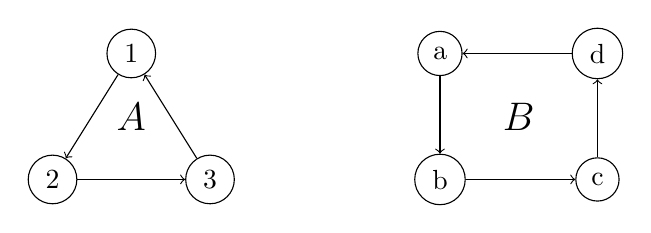
\begin{tikzpicture}[every node/.style={draw,circle}, baseline=(current bounding box.north)]
    \begin{scope}[xshift=-70]
    \node[draw=none, font=\Large] {$\str{A}$};
    \path[->]
      (0,0.8) node(n1) {1}
      (-1,-0.8) node(n2) {2}
      (1,-0.8) node(n3) {3}
      (n1) edge (n2)
      (n2) edge (n3)
      (n3) edge (n1);
    \end{scope}

    \node[draw=none, font=\Large] {$\bisimto_{\GF}$};

    \begin{scope}[xshift=70]
    \node[draw=none, font=\Large] {$\str{B}$};
    \path[->]
      (-1,0.8) node(n1) {a}
      (-1,-0.8) node(n2) {b}
      (1,-0.8) node(n3) {c}
      (1,0.8) node(n4) {d}
      (n1) edge (n2)
      (n2) edge (n3)
      (n3) edge (n4)
      (n4) edge (n1);
    \end{scope}
  \end{tikzpicture}
  \end{figure}
  \vspace{-0.5em}
  \noindent
  By design we clearly have $\str{A}\models \varphi$ and $\str{B} \not\models \varphi$. On the other hand, $\str{A}$ and $\str{B}$ are $\GF$-bisimilar, witnessed by the bisimulation $\bisimZ$ consisting of the partial isomorphisms:
  \begin{itemize}
    \item $(s_{1}, t_{1})$ for every $s_{1} \in \{1,2,3\}$ and $t_{1} \in \{a,b,c,d\}$, and
    \item $(s_{1}s_{2}, t_{1}t_{2})$ for every $s_{1}s_{2} \in \{12,23,31\}$ and $t_{1}t_{2} \in \{ab,bc,cd,da\}$
  \end{itemize}
  where $(s_{1}s_{2}, t_{1}t_{2})$ denotes the partial isomorphism mapping the element $s_{1}$ to $t_{1}$ and the element $s_{2}$ to $t_{2}$.
\end{example}

\clearpage
\section{Bisimulation for $\FGF$}
The notion of bisimulation for $\FGF$ is similar to the one for $\GF$, but takes the ``forwardness'' of $\FGF$ into account.
Due to the ``forwardness'', two tuples which satisfy the exact same atomic formula of $\FGF$ do not necessarily induce a partial isomorphism.
Hence, we now define \emph{forward partial maps}, which exactly represent the properties captured by atomic $\FGF$ formulae.
Let $\elemtuplea \sqin A$ and $\elemtupleb \sqin B$ be tuples with $|\elemtuplea| = |\elemtupleb|$ from structures $\str{A}$ and $\str{B}$.
The pair $(\elemtuplea, \elemtupleb)$ is a \emph{forward partial map} between if $\elemtuplea$ and $\elemtupleb$ are live and $\atp{\FGF}{\str{A}}{\elemtuplea} = \atp{\FGF}{\str{B}}{\elemtupleb}$~holds.
For our fixed signature $\Sigma$, we note that $|\elemtuplea| = |\elemtupleb|$ is smaller or equal to $\arity(\Sigma)$, due to the requirement that these tuples are live.
A \emph{system of forward partial maps} between structures $\str{A}$ and $\str{B}$ is a set of $\mathcal{Z}$ where each element is a forward partial map.

Now, we define bisimulations for $\FGF$ in terms of back-and-forth conditions.
Here, the definition of forward partial maps takes the role of the \ref{sbisim:atomicharmony} condition of basic bisimulations.
\begin{definition}[$\FGF$ back-and-forth conditions and bisimulation]
  For non-empty systems of partial maps $\mathcal{Y}, \mathcal{Z}$ between structure $\str{A}$ and $\str{B}$, we say that $\mathcal{Z}$ satisfies the back-and-forth conditions for $\mathcal{Y}$ if for every forward partial map $(\elemtuplea, \elemtupleb) \in \mathcal{Y}$ we have:
  \begin{description}\itemsep0em
    \item[\desclabel{(fForth)}{bisim:fforth}] For every (possibly empty) infix $\elemtupleafromto{i}{j}$ of $\elemtuplea$ and a live tuple $\elemtuplec$ in $\str{A}$ such that $\elemtupleafromto{i}{j} = \elemtuplecfromto{1}{j{-}i{+}1}$ there is a forward partial map $(\elemtuplec, \elemtupled) \in \mathcal{Z}$ where $\elemtupled$ is a tuple from $\str{B}$ with $\elemtuplebfromto{i}{j} = \elemtupledfromto{1}{j{-}i{+}1}$.
    \item[\desclabel{(fBack)}{bisim:fback}] For every (possibly empty) infix $\elemtuplebfromto{i}{j}$ of $\elemtupleb$ and a live tuple $\elemtupled$ in $\str{B}$ such that $\elemtuplebfromto{i}{j} = \elemtupledfromto{1}{j{-}i{+}1}$ there is a forward partial map $(\elemtuplec, \elemtupled) \in \mathcal{Z}$ where $\elemtuplec$ is a tuple from $\str{A}$ with $\elemtupleafromto{i}{j} = \elemtuplecfromto{1}{j{-}i{+}1}$.
  \end{description}
  A system of forward partial maps $\bisimZ$ between $\str{A}$ and $\str{B}$ is an $\FGF$-\emph{bisimulation} between $\str{A}$ and $\str{B}$ if it itself satisfies the above conditions.
\end{definition}
An $\ell$-$\FGF$-bisimulation between $\str{A}$ and $\str{B}$ is a sequence $\bisimZ_0, \bisimZ_1, \ldots, \bisimZ_\ell$ of systems of forward partial maps between $\str{A}$ and $\str{B}$ such that for all $i < \ell$ we have that $\bisimZ_i$ satisfies~\ref{bisim:fforth} and~\ref{bisim:fback} conditions for $\bisimZ_{i{+}1}$.
We~speak about $\FGF$-\emph{bisimilar} and $\ell$-$\FGF$-\emph{bisimilar} (pointed) structures in total analogy to the guarded-fragment case.
We stress that the back-and-forth conditions allow for choosing an empty infix, so $\ell$-$\FGF$-bisimulations are not limited to the local neighbourhood of some tuple.
Instead, even for $\ell = 1$, every guarded tuple must be mapped to a tuple in the other structure.

Bisimulations for $\FGF$ correspond to logical equivalence with respect to formulae of $\FGF$.
Below, we present a ``forward'' counterpart of \cref{lemma:GF-bisimulations-work-well}.
%!TEX root = ../main.tex

\begin{proof}
  A proof for condition \textbf{(a)} is provided in~\cite[Lemma 3]{BednarczykJ22}, and thus we proceed with condition \textbf{(b)}.
  We start from the ``if'' direction. 
  Let us fix $\sigma$-structures $\str{A}$ and $\str{B}$.
  We want to establish that for all $\ell \in \N$, $\elemtuplea$ in $\str{A}$, and $\elemtupleb$ in $\str{B}$ the following condition holds:
  \[
    (\heartsuit_\ell)(\elemtuplea, \elemtupleb){:} \ \ \ \  (\str{A}, \elemtuplea) \bisimto_{\FGF[\sigma]}^{\ell} (\str{B}, \elemtupleb) \ \text{implies} \ (\str{A}, \elemtuplea) \equiv_{\FGF_\ell[\sigma]} (\str{B}, \elemtupleb).
  \]
  We proceed by induction. 
  For the inductive base, take any $\elemtuplea$ from $\str{A}$, any $\elemtupleb$ from $\str{B}$, and suppose that the antecedent of $(\heartsuit_0)(\elemtuplea,\elemtupleb)$ holds.
  Thus, by \ref{bisim:atomiceq} we know that $\elemtuplea$ and~$\elemtupleb$ have equal $\FGF[\sigma]$-types.
  This means that for all atomic $\varphi$ of $\FGF[\sigma]$ we have $\str{A} \models \varphi[\elemtuplea]$ if and only if $\str{B} \models \varphi[\elemtupleb]$.
  Hence, by a routine case analysis employing obvious properties of $\models$ relation, the above equivalence is lifted to the case of all quantifier-free $\FGF[\sigma]$-formulae, establishing the consequent of $(\heartsuit_0)(\elemtuplea,\elemtupleb)$.
  For the inductive step, fix any positive $\ell$ and assume that for all $k$ smaller than $\ell$ and the condition $(\heartsuit_k)(\elemtuplea,\elemtupleb)$ is satisfied for all tuples $\elemtuplea$ and $\elemtupleb$.
  Now take any tuple $\elemtuplea$ from $\str{A}$ and $\elemtupleb$ from $\str{B}$.
  To show the consequent of $(\heartsuit_\ell)(\elemtuplea,\elemtupleb)$, we take any formula $\varphi(x_1, \ldots, x_n) \in \FGF_\ell[\sigma]$.
  If the quantifier rank of $\varphi$ is smaller than $\ell$, then we are done by $(\heartsuit_{\ell{-}1})(\elemtuplea,\elemtupleb)$.
  Hence, suppose that the quantifier rank of $\varphi$ is precisely~$\ell$.
  By structural induction (relying on properties of $\models$ relation) it amounts to establish the equivalence for $\varphi$ in one of the following forms: 
  \begin{itemize}\itemsep0em

  \item $\varphi$ is of the form $\exists{\vartuplexfromto{n{+}1}{m}}\ \relR(\vartuplexfromto{i}{j}) \land \psi(\vartuplexfromto{i}{j})$, where a predicate $\relR$ serves as a guard, $i \geq 1$ and $j \leq m$.
  Note that the quantifier rank of $\relR(\vartuplexfromto{i}{j}) \land \psi(\vartuplexfromto{i}{j})$ is less than $\ell$.
  Suppose that $\str{A} \models \varphi[\elemtuplea]$ (the case of $\str{B} \models \varphi[\elemtupleb]$ is symmetric).
  Let $\elemtuplec$ be the (possibly empty) infix $\elemtupleafromto{i}{n}$ of~$\elemtuplea$.
  Then there exists a (possibly empty) tuple $\elemtuplee$ in $\str{A}$ such that $\str{A} \models \relR[\elemtuplec\elemtuplee] \land \psi[\elemtuplec\elemtuplee]$.
  Note that $\elemtuplec\elemtuplee$ is $\sigma$-live. 
  By~\ref{bisim:fforth}\bfside{This requires that $\elemtuplea$ is live. Is this true? Example: $\varphi = \relS(x_{1}, x_{2}) \land \relT(x_{3}) \land \exists{x_{4}} (\relH(x_{2}, x_{3}, x_{4}))$ (according to our definitions, this should be an FGF-formula with free variables $x_{1}, x_{2}, x_{3}$, right?) could be satisfied at an $\elemtuplea$ that is not guarded. Perhaps we want to require that the free variables of formulae are guarded as well?} we can find a (possibly empty) tuple $\elemtuplef$ in $\str{B}$ such that $(\str{A}, \elemtuplec\elemtuplee) \bisimto_{\FGF[\sigma]}^{\ell{-}1} (\str{B}, \elemtupled\elemtuplef)$ for~$\elemtupled$ equal to $\elemtuplebfromto{i}{n}$.
  Applying inductive hypothesis, namely $(\heartsuit_{\ell{-}1})(\elemtuplec\elemtuplee,\elemtupled\elemtuplef)$, we know that the consequent of $(\heartsuit_{\ell{-}1})(\elemtuplec\elemtuplee,\elemtupled\elemtuplef)$ holds true.
  This clearly implies $\str{B} \models \relR[\elemtupled\elemtuplef] \land \psi[\elemtupled\elemtuplef]$, which finally lead us to $\str{B} \models \varphi[\elemtupleb]$.

  \item $\varphi$ is of the form $\exists{x_{1}} \psi(x_1)$. Then the quantifier rank of $\psi$ is less than $\ell$.
  Suppose that $\str{A} \models \varphi[\elemtuplea]$ (the case of $\str{B} \models \varphi[\elemtupleb]$ is symmetric).
  Then there exists an element $\elem{c}$ in $\str{A}$ for which $\str{A} \models \psi[\elem{c}]$.
  As $\elem{c}$ is trivially guarded, we apply~\ref{bisim:fforth} to find $\elem{d}$ in $\str{B}$ for which $(\str{A}, \elem{c}) \bisimto_{\FGF[\sigma]}^{\ell{-}1} (\str{B}, \elem{d})$.
  Note that $\ell{-}1$ is non-negative by positivity of $\ell$. 
  Thus, by $(\heartsuit_{\ell{-}1})(\elem{c},\elem{d})$ we know that $(\str{A}, \elem{c}) \equiv_{\FGF_{\ell{-}1}[\sigma]} (\str{B}, \elem{d})$ holds. 
  In particular, this implies $\str{B} \models \psi[\elem{d}]$, concluding the proof.
\end{itemize}

For the opposite direction, take $\ell \in \N$ and a pair of $\omega$-saturated pointed $\sigma$-structures $(\str{A}, \elemtuplea)$ and $(\str{B}, \elemtupleb)$.
Suppose that $(\str{A}, \elemtuplea) \equiv_{\FGF_\ell[\sigma]} (\str{B}, \elemtupleb)$.
We construct a family $\bisimZ_0, \ldots, \bisimZ_\ell$ of systems of forward partial maps as follows:
\[
  \bisimZ_\mathit{k} \coloneqq \{ (\elemtuplec, \elemtupled) \in \bigcup_{i=0}^{\infty} (A^i \times B^i) \mid  (\str{A}, \elemtuplec) \equiv_{\FGF_\mathit{k}[\sigma]} (\str{B}, \elemtupled), \ \text{and} \ \elemtuplec, \elemtupled \ \text{are $\sigma$-live} \}. 
\]
We claim that such a family is an $\ell$-$\FGF[\sigma]$-bisimulation between $(\str{A}, \elemtuplea)$ and $(\str{B}, \elemtupleb)$. 
Note that the condition \ref{bisim:atomiceq} is trivially satisfied by all the $\bisimZ_\mathit{k}$ above, and that $(\elemtuplea, \elemtupleb)$ belongs to all the sets $\bisimZ_\mathit{k}$ by design.
Thus it suffices to show that for all $\mathit{k} \in \{ 1, 2, \ldots, \ell\}$ that the system of forward partial
maps $\bisimZ_\mathit{k}$ satisfies \ref{bisim:fforth} and \ref{bisim:fback} for $\bisimZ_{\mathit{k}{-}1}$.
Hence, take any such $j$ and let us proceed with a proof of \ref{bisim:fforth} (the case of \ref{bisim:fback} is symmetric). 
Let $(\elemtuplec, \elemtupled) \in \bisimZ_\mathit{k}$, $\elemtuplecfromto{i}{j}$ be a (possibly empty) infix of $\elemtuplec$
and $\elemtuplee$ be any tuple in $\str{A}$ such that $\elemtuplecfromto{i}{j}\elemtuplee$ is $\sigma$-live.
We are going to show that the set 
\[
  \Gamma \deff \{ \varphi \mid \str{A} \models \varphi[\elemtuplecfromto{i}{j}\elemtuplee], \varphi \in \FGF_{\mathit{k}{-}1}[\sigma] \}
\] 
is realized in $\str{B}$ by $\elemtupledfromto{i}{j}\elemtuplef$ for some $|\elemtuplee|$-tuple $\elemtuplef$ from $\str{B}$.
By $\omega$-saturation of $\str{B}$ it suffices
to establish that any finite subset of $\Gamma$ is realized by $\elemtupledfromto{i}{j}\elemtupleh$ for some $|\elemtuplee|$-tuple $\elemtupleh$. 
Let $\Delta$ be a finite subset of $\Gamma$.
By design, we have 
$(\str{A}, \elemtuplecfromto{i}{j}) \models \exists{\vartuplex} \textstyle\bigwedge \Delta$.\bbeside{Change $\bar{x}$... Btw, why is this in $\FGF$? Explain. use the guard of $\bar{c}\bar{e}$.}
Moreover, as $\exists{\vartuplex} \textstyle\bigwedge \Delta$ is an $\FGF_\mathit{k}$-formula,
we can invoke $\mathit{k}$-$\FGF$-equivalence of $(\str{A}, \elemtuplec)$ and $(\str{B}, \elemtupled)$ to deduce~$(\str{B}, \elemtupledfromto{i}{j}) \models \exists{\vartuplex} \textstyle\bigwedge \Delta$.
This implies that $\Gamma$ is indeed realized in $\str{B}$, and let $\elemtupledfromto{i}{j}\elemtuplef$ be a tuple witnessing this fact.
By the choice of $\Gamma$, we know that  $(\str{A}, \elemtuplecfromto{i}{j}\elemtuplee) \equiv_{\FGF_{\mathit{k}{-}1}[\sigma]} (\str{B}, \elemtupledfromto{i}{j}\elemtuplef)$, and hence
$(\elemtuplecfromto{i}{j}\elemtuplee, \elemtupledfromto{i}{j}\elemtuplef) \in \bisimZ_{\mathit{k}{-}1}$. 
This concludes the proof of that $\bisimZ_{\mathit{k}}$ satisfies \ref{bisim:fforth}, and thus concludes the proof that the family $\bisimZ_0, \ldots, \bisimZ_\ell$ is an $\ell$-$\FGF[\sigma]$-bisimulation between $(\str{A}, \elemtuplea)$ and $(\str{B}, \elemtupleb)$. 
\end{proof}


\noindent
In the following example, we establish the existence of $\FGF$-bisimilar structures which are not $\GF$-bisimilar.
\begin{example}
  Consider the two structures
  $\str{A} := \tikz[baseline=0.5ex]{\path (0pt,-2.5ex) -- (0pt,-2.5ex); \path[->] (0,0) node[draw,circle] (n1) {a} (n1) edge[loop above,in=70,out=110,looseness=10] (n1);}$ and
  $\str{B} := \tikz[baseline=-0.5ex]{\path[->] (0,0) node (n1) [draw,circle] {1} (3em,0) node (n2) [draw,circle] {2} (n1) edge[bend left] (n2) (n2) edge[bend left] (n1);}$
  with a binary predicate $\relE$ interpreted as the edge relation.
  A $\FGF$-bisimulation between $\str{A}$ and $\str{B}$ is:
  \begin{equation*}
  \mathcal{Z} = \{ (a,1), (a,2), (aa,12), (aa, 21) \}
  \end{equation*}
  This show that these two structures are $\FGF[\{\relE\}]$-bisimilar.
  But the $\GF$-sentence $\exists{\varx_1}\relE(\varx_1,\varx_1)$ can distinguish them, hence they are not $\GF$-bisimilar.
\end{example}

\section{The $\FGF$-bisimulation game}\label{sec:fgf-game}
Both $\GF$-bisimulation and $\FGF$-bisimulation naturally correspond to games~\cite[Sec. 1.2.1]{Gradel014}, which are natural generalizations of the basic bisimulation game.
We focus on the game corresponding to $\FGF$-bisimulation here.
The $\FGF$-\emph{bisimulation game} is played on two pointed structures $(\str{A}, \elemtuplea)$ and $(\str{B}, \elemtupleb)$ by two players, Spoiler and Duplicator.
The game starts by selecting the tuples $\elemtuplea$ and $\elemtupleb$ from the corresponding structures.
Throughout the game, Duplicator must maintain the condition that the two currently selected tuples have equal atomic-$\FGF$-types.
If $\elemtuplea$ and $\elemtupleb$ already do not have the same atomic $\FGF$-type, then Duplicator loses instantly.
Otherwise, the game proceeds in rounds.
In each round, Spoiler first chooses a structure.
As the game is symmetric, let us assume that Spoiler chooses the structure $\str{A}$.
Spoiler then selects an infix $\elemtupleafromto{i}{j}$ of the currently selected tuple $\elemtuplea$ and a fresh live tuple $\elemtuplec$ which has $\elemtupleafromto{i}{j}$ as a prefix.
For convenience, we use the terms \emph{shared elements} for the prefix $\elemtuplecfromto{1}{j-i+1}$ and \emph{unshared elements} for the remaining elements, namely $\elemtuplecfromto{j-i+1+1}{|\elemtuplec|}$.
Duplicator, in order to continue the game, must then find a live tuple $\elemtupled$ in $\str{B}$ having $\elemtuplebfromto{i}{j}$ as prefix such that $\elemtuplec$ and $\elemtupled$ have equal $\FGF$-types.
Note that Spoiler may choose an index $j$ that is not maximal, so that the situation of $a_{j+1} = c_{j-i+1+1}$ is still possible.
We still regard $c_{j-i+1+1}$ as an unshared element, since Duplicator is allowed to pick a tuple $\elemtupled$ where $b_{j+1} \neq d_{j-i+1+1}$.
The game then continues with the next round, with $\elemtuplec$ and $\elemtupled$ as the new starting tuples.
Spoiler wins the game if Duplicator is unable to respond, i.e.\ to find suitable tuples.
Duplicator wins otherwise.
It is easy to see that the possible moves of Spoiler are analogous to the back-and-forth conditions for $\FGF$-bisimulation, as is also the case for the $\GF$-game~\cite[Sec.\ 1.3.2]{Gradel014}.
To win, Duplicator must be able to respond to any move that Spoiler makes.
A winning strategy for Duplicator thus corresponds to an $\FGF$-bisimulation between the two structures, and vice-versa.
If we restrict the game to only $\ell$-rounds, where the winning condition for Duplicator is that Spoiler cannot win in the first $\ell$-rounds, then the game is equivalent (in the aforementioned sense) to the existence of an $\ell$-FGF-bisimulation between $\str{A}, \elemtuplea$ and $\str{B}, \elemtupleb$.
We collect these observations in the following corollary:

\begin{corollary}
  In the $\FGF$-game played on structures $\str{A}, \elemtuplea$ and $\str{B}, \elemtupleb$:
  \begin{itemize}
    \item Duplicator has as winning strategy if and only if $\str{A}, \elemtuplea \bisimto_{\FGF} \str{B}, \elemtupleb$,
    \item Duplicator has a winning strategy for $\ell$ rounds if and only if $\str{A}, \elemtuplea \bisimto_{\FGF}^{\ell} \str{B}, \elemtupleb$.
  \end{itemize}
\end{corollary}

\section{Biseqs and Bipoints}\label{sec:biseqs-and-bipoints}
We next define two concepts (\emph{biseqs} and \emph{bipoints}) which represent a sequence of moves that Spoiler takes and the elements that Spoiler selects, respectively, in one of the possible plays of the $\FGF$-bisimulation game.
Later, in \cref{chap:unraveling}, we employ these concepts to characterize a structure in terms of its behavior under the game.

Let $\str{A}, \elemtuplea^{(0)}$ be a pointed structure where $\elemtuplea^{(0)}$ is just tuple of elements from $A$, labelled with a zero index as it is the start of a sequence of tuples selected by Spoiler.
An $\ell$-\emph{biseq} ($\ell$-bisimimulation sequence) is a word in $A^*{(\N\N{}A^{*})}^{\ell}$, written as a sequence of the form $\elemtuplea^{(0)}(i^{(1)}, j^{(1)})\elemtuplea^{(1)}\cdots(i^{(\ell)}, j^{(\ell)})\elemtuplea^{(\ell)}$, where each $a^{(k)}$ is a live tuple from $\str{A}$ and $i^{(k)}, j^{(k)}$ are indices with $i \le j$ for which $\elemtupleafromto{i^{(k)}}{j^{(k)}}^{(k-1)} = \elemtupleafromto{1}{j^{(k)}-i^{(k)}+1}^{k}$.
Conceptually, an $\ell$-biseq represents a play of Spoiler in the $\ell$-round $\FGF$-game involving the structure $\str{A}$, where in each round $k$, Spoiler chooses the non-empty infix corresponding to the indices $i^{(k)}\ldots{}j^{(k)}$ and the new tuple $\elemtuplea^{(k)}$.
Biseqs are denoted by greek letters $\rho, \sigma, \theta, \ldots$ and for
a biseq $\sigma$ we refer to the parameter $\ell$ in the above definition as the \emph{level} of $\sigma$.
We say that a biseq $\sigma$ \emph{extends} a biseq $\rho$ if $\sigma$ can be constructed from $\rho$ by adding moves to the end, \ie{} if $\rho$ is a prefix of $\sigma$.
The set of all biseqs for a structure $\str{A}$, denoted by $\Seq{A}$, intuitively collects all possible ways in which Spoiler can explore this structure.
For any $\ell$-biseq, if $\str{B}, \elemtupleb^{(0)}$ is a structure that is \FGF-bisimilar to $\str{A}, \elemtuplea^{(0)}$, then we can apply~\ref{bisim:fforth} $\ell$ times to find tuples $\elemtupleb^{1}, \ldots, \elemtupleb^{\ell}$ for a corresponding biseq in $\str{B}$.
The latter sequence represents a possible choice of moves for Duplicator in response to the moves played by Spoiler in the game on the structures $\str{A}, \elemtuplea^{(0)}$ and $\str{B}, \elemtupleb^{(0)}$. The example on the following page illustrates the definition of biseqs.\clearpage

\begin{example}\label{fig:biseq-examples}
  \mbox{}\\
  \hfill{}\begin{minipage}[t]{0.2\textwidth}
      \raggedleft%
      \vspace{0pt}
      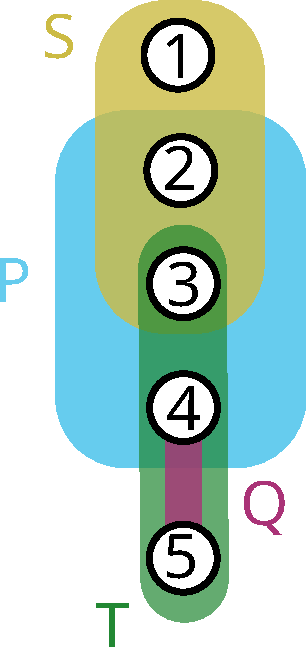
\includegraphics[scale=0.5]{res/example-struct-1}
  \end{minipage}
  \hspace{4em}
  \begin{minipage}[t]{0.6\textwidth}
    {%
    \newcommand{\tups}{{\color{tolbrightYellowDarker}\elemtuples}}%
    \newcommand{\tupp}{{\color{tolbrightCyanDarker}\elemtuplep}}%
    \newcommand{\tupt}{{\color{tolbrightGreen}\elemtuplet}}%
    \newcommand{\tupq}{{\color{tolbrightPurple}\elemtupleq}}%
    The picture on the left shows a structure with the relations: $(1,2,3) \in \relS^{\str{A}}$, $(2,3,4) \in \relP^{\str{A}}$, $(3,4,5) \in \relT^{\str{A}}$, $(4,5) \in \relQ^{\str{A}}$.

    \vspace{1ex}
    Let $\tups = (1, 2, 3)$, $\tupp = (2, 3, 4)$, $\tupt = (3, 4, 5)$ and $\tupq = (4,5)$.

    \vspace{1ex}
    Some examples of biseqs in this structure are:
    \begin{itemize}
        \item $\tups(3,3)\tupt$, and
        \item $\tups(2,3)\tupp(2,3)\tupt$.
    \end{itemize}

    Biseqs are not required to use maximal infixes, so the following are also valid biseqs:
    \begin{itemize}
        \item $\tups(2,2)\tupp$, and
        \item $\tups(3,3)\tupt(2,2)\tupq$.
    \end{itemize}
    }
  \end{minipage}
  \hfill{}\\
\end{example}

Let $\Seq{\str{A}}$ be the set of all biseqs for a structure $\str{A}$.
There is a natural projection $\Pi$ from a biseq $\sigma \in \Seq{A}$ to tuples of $\str{A}$: for $\sigma = \cdots (i,j) \elemtuples$, we define $\Pi(\sigma)$ to be $\Pi(\sigma) = \elemtuples$.
Intuitively, this projection gives the tuple of selected elements in structure $\str{A}$ in the bisimulation game after playing the moves of $\sigma$.
We now introduce ``bipoints'', which have a projection to individual selected elements (``points'') of $\str{A}$ instead.
A \emph{bipoint} of a structure $\str{A}$ is a tuple $(\sigma, k) \in \Seq{A} \times \mathbb{N}$ such that either
\begin{itemize}
  \item $\sigma = \elemtuplea$, for some $\elemtuplea \sqin A$ where $1 \le k$ and $k \le |\elemtuplea|$, or
  \item $\sigma = \cdots (i,j) \elemtuplea$, for some $\elemtuplea \sqin A$ where $(j-i+1) + 1 \le k$ and $k \le |\elemtuplea|$ .
\end{itemize}
For a bipoint $e$ of a structure $\str{A}$ that can be decomposed as $e = (\rho, k)$, we use the notation $\seq{e} = \rho$ and $\ctr{e} = k$ to denote the biseq and the counter of this bipoint, respectively.
The counter of the bipoint identifies one component of the tuple of elements that the biseq projects to.
We define the projection $\pi$ from bipoints of a structure $\str{A}$ to elements of $\str{A}$ as follows: if $e = (\sigma, k)$ is a bipoint, then $\pi(e) = {\Pi(\sigma)}_{k}$ (which is equal to $\elema_{k}$ in case $\sigma = \cdots\elemtuplea$).
The condition ``$k \ge (j-i+1) + 1$'' ensures that we do not have more than one bipoint for the shared elements in a move in the bisimulation game.
\Cref{ex:bipoints} shows a concrete application for this condition.

\begin{example}\label{ex:bipoints}
   {%
     \newcommand{\tups}{{\color{tolbrightYellowDarker}\elemtuples}}%
     \newcommand{\tupt}{{\color{tolbrightGreen}\elemtuplet}}%
     \newcommand{\es}{{\color{tolbrightYellowDarker}s}}%
     \newcommand{\et}{{\color{tolbrightGreen}t}}%
     Consider the biseqs from \cref{fig:biseq-examples}.
     The bipoints for the 0-biseq $\sigma$ with $\sigma = \tups$ are: $a = (\sigma, 1)$, $b = (\sigma, 2)$ and $c = (\sigma, 3)$.
     These project to the components of the tuple $\tups$: $\pi(a) = \es_{1} = 1$, $\pi(b) = \es_{2} = 2$ and $\pi(c) = \es_{3} = 3$.
     Now consider the 1-biseq $\rho$ with $\rho = \tups(3,3)\tupt$.
     Regarded in terms of the game, this sequence represents the move from $\tups$ to $\tupt$, sharing the element ``3''.
     There are bipoints $d = (\rho, 2)$ and $e = (\rho, 3)$ which project to the domain elements ``4'' and ``5''.
     However, there is no bipoint for the sequence $\rho$ that projects to ``3''.
     While $(\rho, 1)$ projects to ``3'' according to the definition of $\pi$, it is not a bipoint as it violates the ``$k \ge (j-i+1) + 1$'' condition in the above definition.
     Note that $c = (\sigma, 3)$ projects to ``3'', so there already is a bipoint that projects to ``3'', using the sequence $\sigma$.
     In fact, bipoints correspond one-to-one to unshared elements of moves in the bisimulation game.
     From the point of view of the biseq $\sigma$, the element ``3'' is not shared with previously selected elements (there are none, since $\sigma$ represents the start of the game at tuple $\tups$), while relative to the biseq $\rho$, the element ``3'' is among the shared elements.
     Hence, $(\sigma, 3)$ is a bipoint, while $(\rho ,1)$ is not.
   }
\end{example}
